\chapter{Arquitectura}\label{diseno}
En este capítulo se explicará la arquitectura general del sistema y sus componentes principales: el servicio de localización, el servicio \textit{Backend} y la aplicación \textit{iOS}.

\section{Arquitectura general del sistema}

\begin{figure}[tbp]
\centering
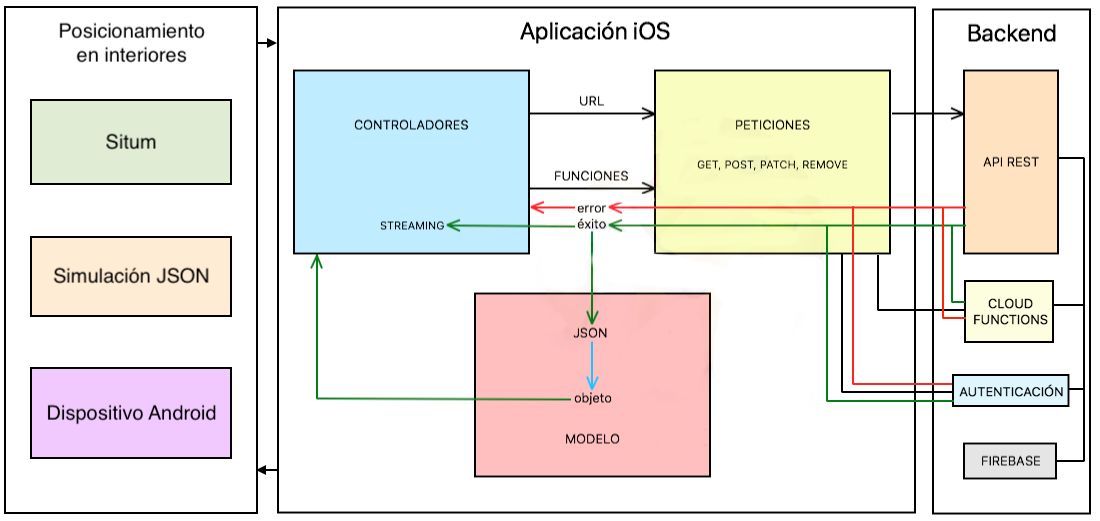
\includegraphics[width=\textwidth]{figures/arquitectura.png}
\caption{Arquitectura general de nuestro sistema de publicidad geolocalizada.\label{fig:arquitectura_2}}
\end{figure}

El sistema está compuesto de tres módulos principales (figura~\ref{fig:arquitectura_2}).
\begin{enumerate}
\item \textbf{\textit{Backend}.} Se ha utilizado la plataforma \textit{Firebase} para desarrollar este módulo. Utilizando los servicios de base de datos en tiempo real, autenticación y \textit{Cloud Functions}.

\item \textbf{Geolocalización.} Es el módulo encargado de determinar la posición del teléfono móvil (y por tanto del usuario)tanto en interiores como en exteriores.

\item \textbf{\textit{Frontend}.} Aplicación \textit{iOS} que se comunica con los otros dos módulos y que permite al usuario interaccionar con la plataforma. 
Se han definido diferentes roles para tener acceso a las distintas acciones previstas en cada caso.
\end{enumerate}

\section{Servicio de localización}
Como se puede observar en la figura~\ref{fig:arquitectura}, el servicio de localización determina la posición del teléfono móvil a partir de los datos que ésta le manda.
Los datos que necesita son el GPS (para la posición en el exterior), los sensores inerciales (acelerómetro, giróscopo y magnetómetro), la información de \emph{Bluetooth} (típicamente balizas fijadas en el edificio) y los datos sobre las redes Wifi detectadas. 
La información sobre la posición se envía directamente a la aplicación \emph{iOS}.

En nuestro prototipo hemos empleado la tecnología de \textit{Situm}.
Se integra su librería en la propia aplicación, y una vez autenticada mediante un código, ella ya se encarga de obtener la información de los servidores de \emph{Situm} (mapas, calibraciones, etc) y de ir obteniendo la información de los sensores y calculando la posición del móvil.


\begin{figure}[tbp]
\centering
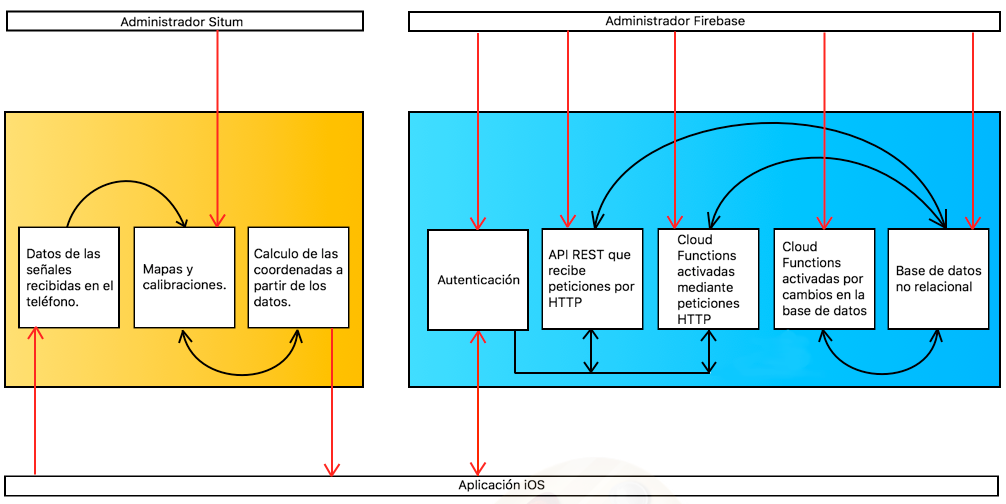
\includegraphics[width=\textwidth]{figures/Untitled2.png}
\caption{Arquitectura general de nuestro sistema de publicidad geolocalizada.\label{fig:arquitectura}}
\end{figure}

El administrador de la plataforma es el único que tiene acceso a la cuenta de \textit{Situm}, de tal manera que debe ser él el que suba las calibraciones y los mapas. Esto puede ser un problema, ya que cada vez que un gestor de centro comercial quiera subir sus mapas o calibraciones tendrá que pasar por el administrador de la plataforma. Quizás en el futuro, los de \textit{Situm} creen una funcionalidad que permita subir mapas y calibraciones a una cuenta, sin necesidad de ser propietarios de la misma.



\subsection{Simulación\label{sec:simul_subsec}}

La tecnología de la localización en interiores en el sistema operativo \emph{iOS} es un tema delicado, porque desde hace ya varios años, \emph{Apple} no da acceso a la información de la Wifi. De esa manera, la tecnología de \emph{Situm} para \emph{iOS} depende exclusivamente de la información de las balizas \emph{Bluetooth} fijadas en el entorno.

En nuestro caso, no teníamos a nuestra disposición ningún edificio calibrado con balizas. Y debido al coste y a las complicaciones del despliegue (robos, etc.) no nos planteamos calibrar ningún edificio por nuestros propios medios.

Por lo tanto, hemos pensado en desarrollar otras alternativas (ver figura~\ref{fig:arquitectura}) para probar el prototipo del sistema. 
La primera opción era desarrollar una aplicación Android (ejecutándose en un dispositivo Android) que ``acompañase'' al usuario con móvil \emph{iOS}. De esta forma, se podrían usar cualquier tipo de edificio con Wifis, por ejemplo la propia Facultad de Informática. 
Al final se descartó por ser poco operativo.

La segunda opción era simular el movimiento del propio móvil.
Las ventajas era la sencillez y la facilidad de uso.
Por desgracia, en \emph{iOS} no se puede simular la información de posición. Además, \emph{Situm} aún no tenía finalizada esta característica en su librería, por lo tuvimos que interaccionar con ellos para implementarla en nuestra aplicación.

Se escogió utilizar un fichero JSON con coordenadas que representaban las distintas posiciones de un usuario a lo largo de una ruta por un centro comercial. Este método era el más sencillo, sobre todo porque podíamos trabajar y hacer pruebas sin necesidad de levantarnos de la silla.


\section{Servicio de \textit{Backend}}
En esta sección se hablará sobre los servicios de la plataforma \textit{Firebase} que fueron utilizados a lo largo de la realización de este proyecto; autenticación, \textit{API REST}, \textit{Cloud Functions} y sus implicaciones sobre el modelo de datos.

\subsection{Autenticación}
Podemos observar en la figura~\ref{fig:arquitectura} que para comunicarnos con \textit{Firebase}, la aplicación debe pasar primero siempre por un proceso de autenticación. Como hemos utilizado la \textit{API REST}, debíamos añadir a toda \textit{URL} la \textit{query-string} \textbf{\textit{key=[API\_KEY]} }\cite{noauthor_firebase_nodate-1}. Este \textit{API\_KEY} es un \textit{token} que se le proporciona al usuario cuando inicia sesión mediante alguno de los múltiples métodos soportados: \textit{Google}, \textit{Twitter}, \textit{Facebook} u otros \cite{noauthor_users_nodate}.

También será necesario ajustar las reglas de \textit{Firebase} a nuestro gusto. Dependiendo de si sólo se quieren permitir las lecturas y las escrituras a usuarios autenticados (ver código~\ref{list:rules-auth}), o si por motivos de comodidad o para realizar alguna prueba, nos interesa desactivar la autenticación y permitir lecturas y escrituras a cualquiera (ver código~\ref{list:rules-true}). Pero las reglas de \textit{Firebase} permiten hacer muchas más cosas, hay una amplia documentación al respecto \cite{noauthor_firebase_nodate}.

\begin{lstlisting}[language=json,style=interfaces,caption=Reglas Firebase que exigen estar autenticado para hacer cambios.,label={list:rules-auth}]
{
  "rules":
  {
    ".read": "auth != null",
    ".write": "auth != null"
  }
}
\end{lstlisting}

\begin{lstlisting}[language=json,style=interfaces,caption=Reglas Firebase que permiten leer y escribir a cualquier usuario.,label={list:rules-true}]
{
  "rules":
  {
    ".read": true,
    ".write": true
  }
}
\end{lstlisting}

\subsection{\textit{API REST}}
Para acceder a los datos se ha decidido utilizar una \textit{API REST}, debido a que este método soporta todas las funcionalidades necesarias para el desarrollo del proyecto y además es uno de los más extendidos. De modo que, al igual que con los servicios de localización, aquí tenemos otra caja negra que nos permitirá adaptarnos fácilmente el día que decidamos cambiar de servidores.

Como se aprecia en la figura \ref{fig:arquitectura}, este componente del sistema recibe una petición del usuario autenticado, escribe y/o lee de la base de datos y finalmente devuelve una respuesta a dicho usuario.

\subsection{\textit{Cloud Functions}}\label{cloud:section}
En esta sección comentaremos los dos tipos de \textit{Cloud Functions} utilizadas y sus diferencias a la hora de integrarse con el resto de componentes de la plataforma.

\subsubsection*{\textit{Cloud Functions} activadas mediante peticiones \textit{HTTP}}
Estas funciones tienen asociada una \textit{URL}, se ejecutan mediante una petición \textit{HTTP} de un usuario autenticado. Leen y/o escriben la base de datos y pueden devolver una respuesta a dicho usuario, como muestra el esquema \ref{fig:arquitectura}.

Para cambiar \textit{Firebase} por otra plataforma o por nuestros propios servidores, el único cambio que habría que hacer en la aplicación \textit{iOS} sería la \textit{URL}.

\subsubsection*{\textit{Cloud Functions} activadas tras cambios en la base de datos}
Estas funciones se ejecutan sin intervención del usuario, se vinculan con un determinado nodo de la base de datos de manera que se lanzan cuando se produce un cambio en el mismo (esquema de la figura~\ref{fig:arquitectura}). Estarían aisladas de los demás componentes del proyecto, si un día quisieramos cambiar de servidores, añadir, eliminar o modificar alguna de estas funciones en caliente, no habría que tocar en absoluto la aplicación \textit{iOS}.

\subsection{Modelo de datos}
Al ser una base de datos no relacional en formato \textit{JSON}, nos quedaría una estructura de árbol con varios niveles (ver código~\ref{list:tree-nosql}). Si tratásemos de hacer lo mismo con un modelo relacional nos quedaría un esquema como el de la figura~\ref{fig:modelo}.

\begin{lstlisting}[language=json,style=interfaces,caption=Árbol formado por una base de datos no relacional.,label={list:tree-nosql}]
"Buildings" : {
  "3598" : {
  	"Managers" : {
  		"-4712897510522395898" : {
  			"Email" : "gestor.centro.comercial@gmail.com"
		}
  	},
  	"Shops" : {
  		"-LKnOeINwIY7m0wEfK90" : {
  			"Name" : "Cafeteria",
  			"Offers" : {
  				"-LKnTA635eXVIBDOxQpt" : {
  					"Description" : "Croissant, zumo y Colacao",
  					"Floor" : 1,
  					"Latitude" : 43.3328167533505,
  					"Longitude" : -8.411021903157234,
  					"Radius" : 20,
  					"Title" : "Desayuno 2 euros",
  					"expiration" : "1535494759171.4001",
  					"quantity" : "10"
				}
  			}
  		}
  	}
}
\end{lstlisting}

\begin{figure}[tbp]
\centering
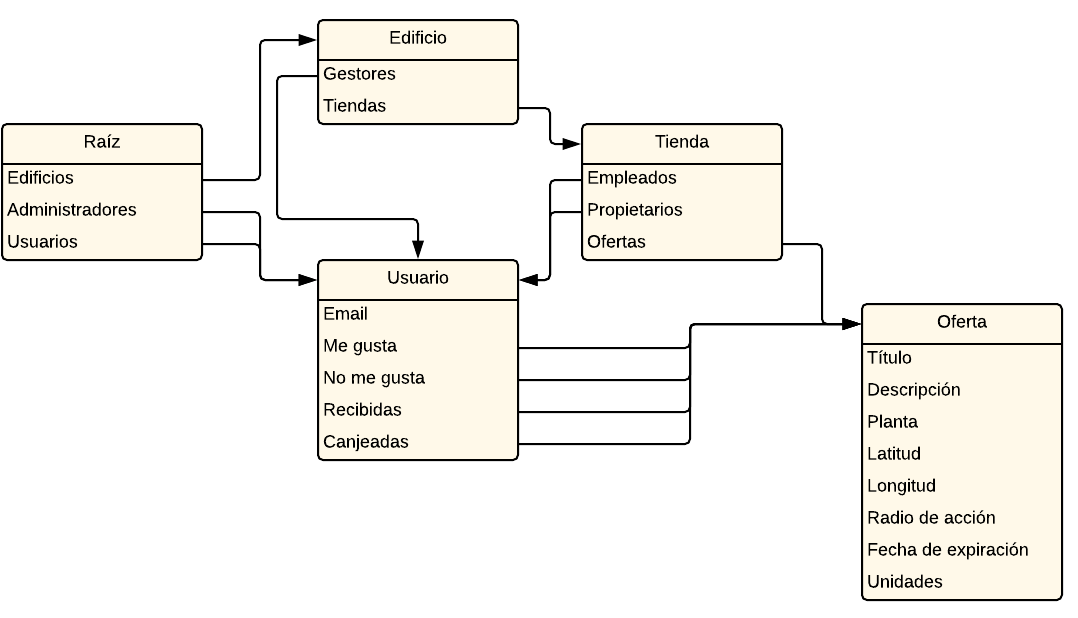
\includegraphics[scale=0.35]{figures/modelo.png}
\caption{Modelo de datos del servicio \emph{Backend}.
 Por comodidad, se representa el modelo de una base de datos relacional equivalente.\label{fig:modelo}}
\end{figure}

\subsubsection*{Limitaciones de una base de datos \textit{NoSQL}} \label{nosql}
Una base de datos no relacional, no se estructura de la misma manera que una que sí lo es (figura~\ref{fig:nosqlVS}). Por ejemplo, en esta aplicación tenemos las ofertas, que se encuentran dentro de una tienda y que a su vez se encuentran dentro de un edificio. Pero cuando un usuario indica que le gusta una oferta, la información se guarda en su perfil, no en la oferta. Surge aquí un problema, porque quizás queramos datos que ya están almacenados en el propio nodo de la oferta, pero los queremos accesibles desde el nodo del usuario.

Este proyecto nació con la idea de utilizar solamente el servicio de base de datos de \textit{Firebase}, así que en situaciones como estas no hubo más opciones que replicar datos. Lo cual es muy ineficiente, siendo la otra opción almacenar la \textit{URL} de la oferta en el nodo del usuario y realizar una petición extra, pero esto aumentaría el consumo de datos en el teléfono móvil de los usuarios.

\subsubsection*{Aparición de \textit{Cloud Functions}}
Poco a poco fueron apareciendo nuevas necesidades en el proyecto, que obligaron a utilizar \textit{Cloud Functions}. La capacidad de ejecutar código en un servidor permite cambiar por completo la arquitectura de una base de datos de este tipo. Ya que para solucionar el problema anteriormente comentado de los \textit{me gusta}, el usuario solamente con una petición podría bajarse las ofertas de la tienda ya con su información personal. Sin necesidad de replicar datos ni de hacer varias peticiones, la función de \textit{Cloud Functions} recibiría la petición, realizaría las búsquedas pertinentes en la base de datos, compondría el listado de ofertas con datos del usuario y se la devolvería al cliente.

\begin{figure}[tbp]
\centering
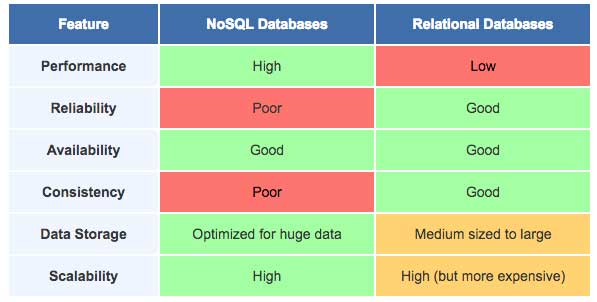
\includegraphics[scale=0.5]{figures/nosqlVS.jpg}
\caption{Relacional VS No relacional.\label{fig:nosqlVS}}
\end{figure}

\section{Arquitectura de la aplicación móvil: MVC}
Para el desarrollo de la aplicación \textit{iOS} se ha utilizado el patrón Modelo Vista Controlador. La herramienta \textit{Xcode}, nos permite crear aplicaciones \textit{iOS} mediante este patrón de diseño.
En la figura~\ref{fig:arq_ios} se puede ver la arquitectura de la aplicación \emph{iOS}. A continuación, explicaremos cada uno de los elementos: modelo (datos y peticiones), vista y controlador. 

\begin{figure}[tb]
\centering
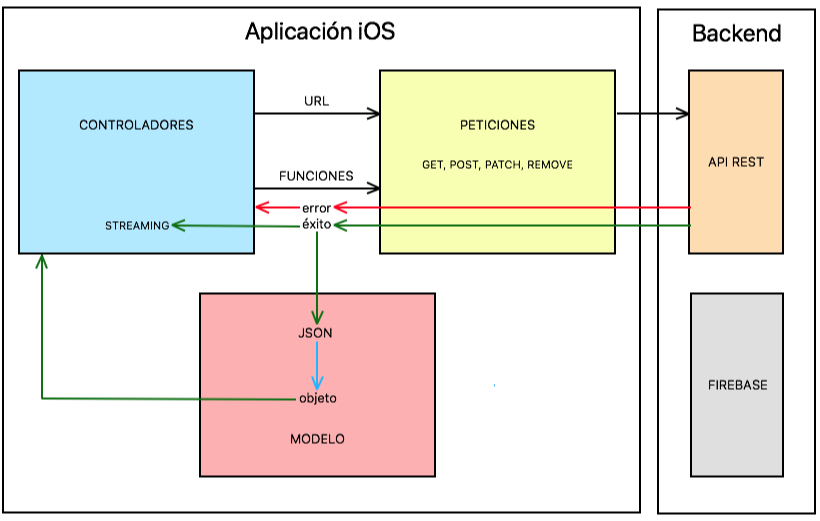
\includegraphics[width=0.89\textwidth]{figures/esquema-impl.png}
\caption{Arquitectura general de la aplicación \emph{iOS}.\label{fig:arq_ios}}
\end{figure}

\subsection{Modelo}
En esta subsección hablaremos de como se organiza la aplicación para obtener los datos de \textit{Firebase}.

\paragraph{Peticiones.}
Se separan del resto del código, las funciones utilizadas para comunicarse con la base de datos. Por ejemplo, si queremos pedir una oferta determinada, simplemente ejecutamos la función correspondiente, la cual nos devolverá dicha oferta. Las peticiones se organizan en clases (figura~\ref{fig:peticiones}) y cada función se define como un método estático, de esta manera pueden ser llamadas desde cualquier otra clase sin necesidad de crear una instancia, esto ofrece varias ventajas.

\begin{itemize}
\item{}\textbf{Reutilización de código.} Una petición, por ejemplo para obtener una oferta determinada, es probable que se vaya a llamar desde multitud de clases.

\item{}\textbf{Modificaciones y errores.} Si una petición no está funcionando como se esperaba o queremos modificar algo. Será mucho más fácil arreglar el problema si la tenemos aislada y localizada, evitándonos buscar todas las veces que se hace la petición por todo el código.
\end{itemize}

\subsubsection*{Programación orientada a objetos}
Todos los nodos que recuperemos de la base de datos deberán mapearse en clases para poder así trabajar con ellos. El modelo de datos de la figura~\ref{fig:modelo}, daría lugar a las clases que vemos en la figura~\ref{fig:objetos}.

\begin{figure}[tbp]
\centering
\subfigure{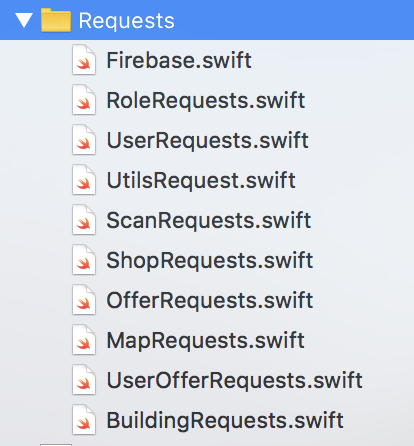
\includegraphics[scale=0.6]{figures/peticiones.png}\label{fig:peticiones}}
\subfigure{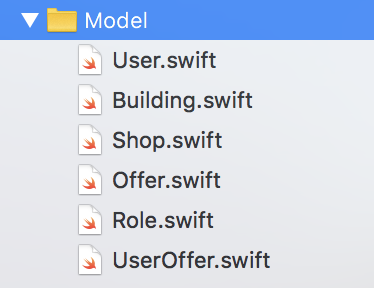
\includegraphics[scale=0.6]{figures/objetos.png}\label{fig:objetos}}
\caption{Modelo \textit{app}: (a) Aislamiento de peticiones y (b) clases de la aplicación.}
\end{figure}

\subsection{Vista}

\begin{figure}[t]
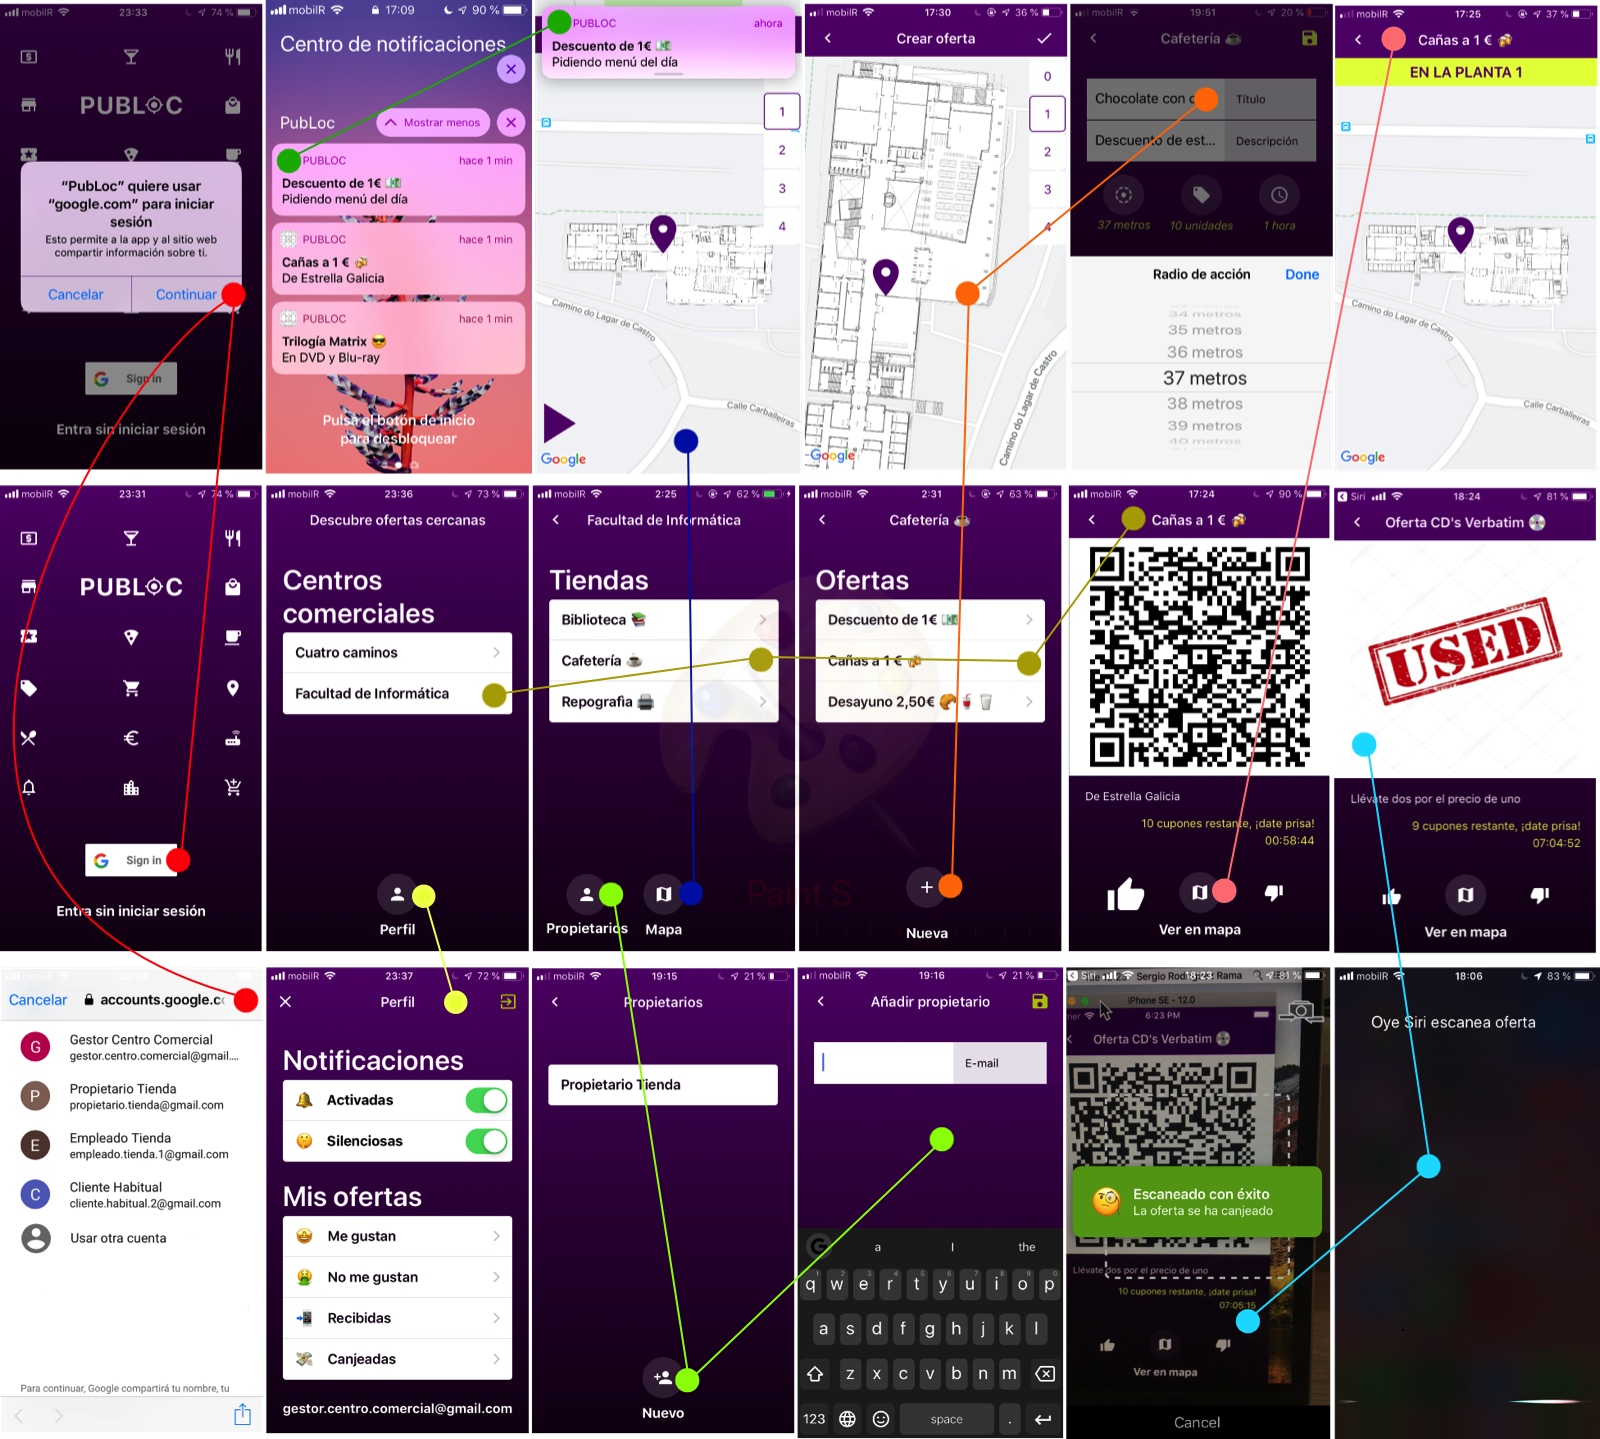
\includegraphics[width=\textwidth]{figures/esquema2.png}
\captionsetup{singlelinecheck=off,font=footnotesize}
\caption[Conjunto de las vistas diseñadas en la aplicación \emph{iOS} agrupadas por temática.]{Conjunto de las vistas diseñadas en la aplicación \emph{iOS} agrupadas por temática:
\legendbox{mi_rojo} Autenticación,
\legendbox{mi_dorado} Datos generales (centros comerciales, tiendas y ofertas), 
\legendbox{mi_verde} Notificaciones,
\legendbox{mi_azul_oscuro} Mapa de edificio, 
\legendbox{mi_naranja} Nueva oferta,
\legendbox{mi_rosa_pastel} Mapa de oferta,
\legendbox{mi_amarillo_claro} Perfil,
\legendbox{mi_verde_claro} Crear rol,
\legendbox{mi_celeste} Escaneo de códigos \textit{QR}.\label{fig:esquema2}}
\end{figure}

En la figura~\ref{fig:esquema2} podemos ver como se ha estructurado la vista de la aplicación, las diferentes pantallas y como se relacionan entre ellas.

\paragraph{Autenticación.} Pantalla incial de la aplicación, con dos botones. Uno para iniciar sesión con \textit{Google} y otro para entrar a la aplicación directamente. Si seleccionamos iniciar sesión con \textit{Google} se nos redirigirá automáticamente al selector de cuentas y cuando se termine la autenticación, podremos visualizar los centros comerciales.

\paragraph{Datos generales.} Estas pantallas contienen los listados de centros comerciales, tiendas y ofertas, hasta llegar al detalle de la oferta donde se encuentra el código \textit{QR}. Dependiendo de los roles que tenga el usuario, las acciones \textit{CRUD} de roles, ofertas y tiendas le serán visibles o no.

\paragraph{Notificaciones.} Cuando el usuario entra en el radio de acción de una oferta, salta una notificación y se puede visualizar tanto con la \textit{app} abierta como con el móvil bloqueado, en la parrilla de notificaciones.

\paragraph{Mapa de edificio.} Desde la pantalla que contiene las tiendas de un centro comercial, podemos ver su mapa. Desde él, veremos nuestra posición en el plano, pudiendo seleccionar cualquiera de las plantas que tiene el edificio para ver las ofertas que hay en ella.

\paragraph{Nueva oferta.} Desde la pantalla que contiene las ofertas de una tienda, podemos añadir una nueva oferta. Tendríamos que darle un nombre, una descripción, un radio de acción, una duración y un límite de unidades disponibles. Es necesario tener rol de propietario de dicha tienda para poder llevar a cabo esta acción.
Las pantallas de creación de tienda no aparecen en el esquema porque sería muy similar a éstas, la única diferencia es que el único atributo de las tiendas es su nombre.

\paragraph{Mapa de oferta.} Desde la pantalla de detalle de una oferta, podemos ver su posición en el mapa. Se mostrará la planta del edificio que la contiene y no habrá botones que nos permitan explorar las demás.

\paragraph{Perfil.} Aquí se pueden silenciar o desactivar las notificaciones y también ver las ofertas del usuario: favoritas, rechazadas, recibidas y canjeadas. Si seleccionamos cualquiera de estas, se mostrará una lista de ofertas similar a la que mostrábamos al seleccionar una tienda.

\paragraph{Crear rol.} Las pantallas de creación de rol son idénticas para cualquier rol que creamos crear, simplemente será necesario introducir el \textit{email} de un usuario autenticado en la plataforma para asignarle el rol en cuestión. Estas funcionalidades no estarán visibles para todos los usuarios de la aplicación, sólo para aquellos que tengan los permisos necesarios.

\paragraph{Escaneo de códigos \textit{QR}.} El escáner de códigos \textit{QR} puede lanzarse desde un botón que hay en perfil de usuario, pero también se puede abrir utilizando atajos de \textit{Siri} y funciona aunque la aplicación esté cerrada. Cuando se realiza un escaneo, se proporciona siempre \textit{feedback} al empleado de la tienda, mostrándole un aviso por pantalla.

\subsubsection*{Sinergia entre el modelo y la vista}
Aunque el modelo y la vista están separados según el patrón Modelo-Vista-Controlador, puede pasar que la propia estructura de la base de datos condicione la interfaz de usuario. Como vimos en la sección  \ref{nosql}, hay una separación entre datos de perfil y datos generales de la aplicación. Un ejemplo de como podría afectar esta arquitectura a la interfaz de usuario sería el siguiente:

Imaginemos que se quiere que los botones \textit{like}/\textit{dislike}  vayan incorporados en las celdas de la tabla de ofertas de una tienda. Como este proyecto nació con la idea de utilizar la base de datos que ofrece \textit{Firebase} únicamente, comunicándonos con ella mediante \textit{API REST}; para lograr esto, a la hora de elaborar la tabla deberíamos tener acceso a las ofertas de la tienda y a las ofertas del usuario para compararlas y saber que opinión tiene el usuario al respecto de cada una de ellas. Esto no solamente obligaría a hacer una petición extra, sino que también obligaría al terminal móvil del cliente a trabajar de más: almacenando dos listas de ofertas en lugar de una, comparándolas y creando una a partir de ambas.

Para darle solución a este problema, se decidió poner los botones de \textit{like}/\textit{dislike} situados en el detalle de la oferta, en lugar de tenerlos en cada celda de la tabla. De esta manera sólo se descargaría la información de usuario de una oferta determinada cada vez que entramos en ella, en lugar de tener que pedirlas todas para filtrar las ofertas de la tienda.

Más tarde, surgió la necesidad de incluir \textit{Cloud Functions} en el proyecto y apareció la posibilidad de incluir los botones en las celdas, pero se decidió no abordar este cambio de diseño por falta de tiempo y dejarlo para futuras iteraciones.

\subsection{Controlador}
El controlador funciona como intermediario entre la vista y el modelo, cambios en el modelo que tendrán su efecto en la vista y acciones en la vista que tendrán su efecto en el modelo, serán gestionados por el controlador. Las aplicaciones \textit{iOS} se construyen basándose en el patrón Modelo-Vista-Controlador, a continuación explicaremos como se estructuran los diversos controladores que componen una aplicación.

\subsubsection*{Controlador padre}
No es obligatorio, pero es recomendable comenzar toda aplicación \textit{iOS} con un controlador padre, conocido como \textit{UINavigationController}. Tendrá una pila en la cual se irán añadiendo controladores hijos y él será el encargado de gestionar las transiciones entre ellos y la navegación a través de las diversas pantallas de la aplicación.

\paragraph{\textit{Push}.} Consiste en añadir un nuevo controlador hijo a la pila, el cual se convertirá en el controlador visible (el que verá y con el interactuará el usuario). Si se animase la transición, la nueva pantalla aparece en escena por defecto deslizándose de derecha a izquierda (en árabe, de izquierda a derecha).

\paragraph{\textit{Pop}.} Consiste en sacar de la pila el último controlador hijo añadido, convirtiéndose el siguiente de la pila en el controlador visible. Esta acción es más conocida como \textit{Atrás} y suele representarse con un botón con una flecha en la parte superior izquierda (en árabe, la derecha). También suele realizarse esta acción deslizando el dedo en la dirección contraria al \textit{push} desde el borde de la pantalla, ver figura~\ref{ref:pop-push}.

\begin{figure}[tbp]
\centering
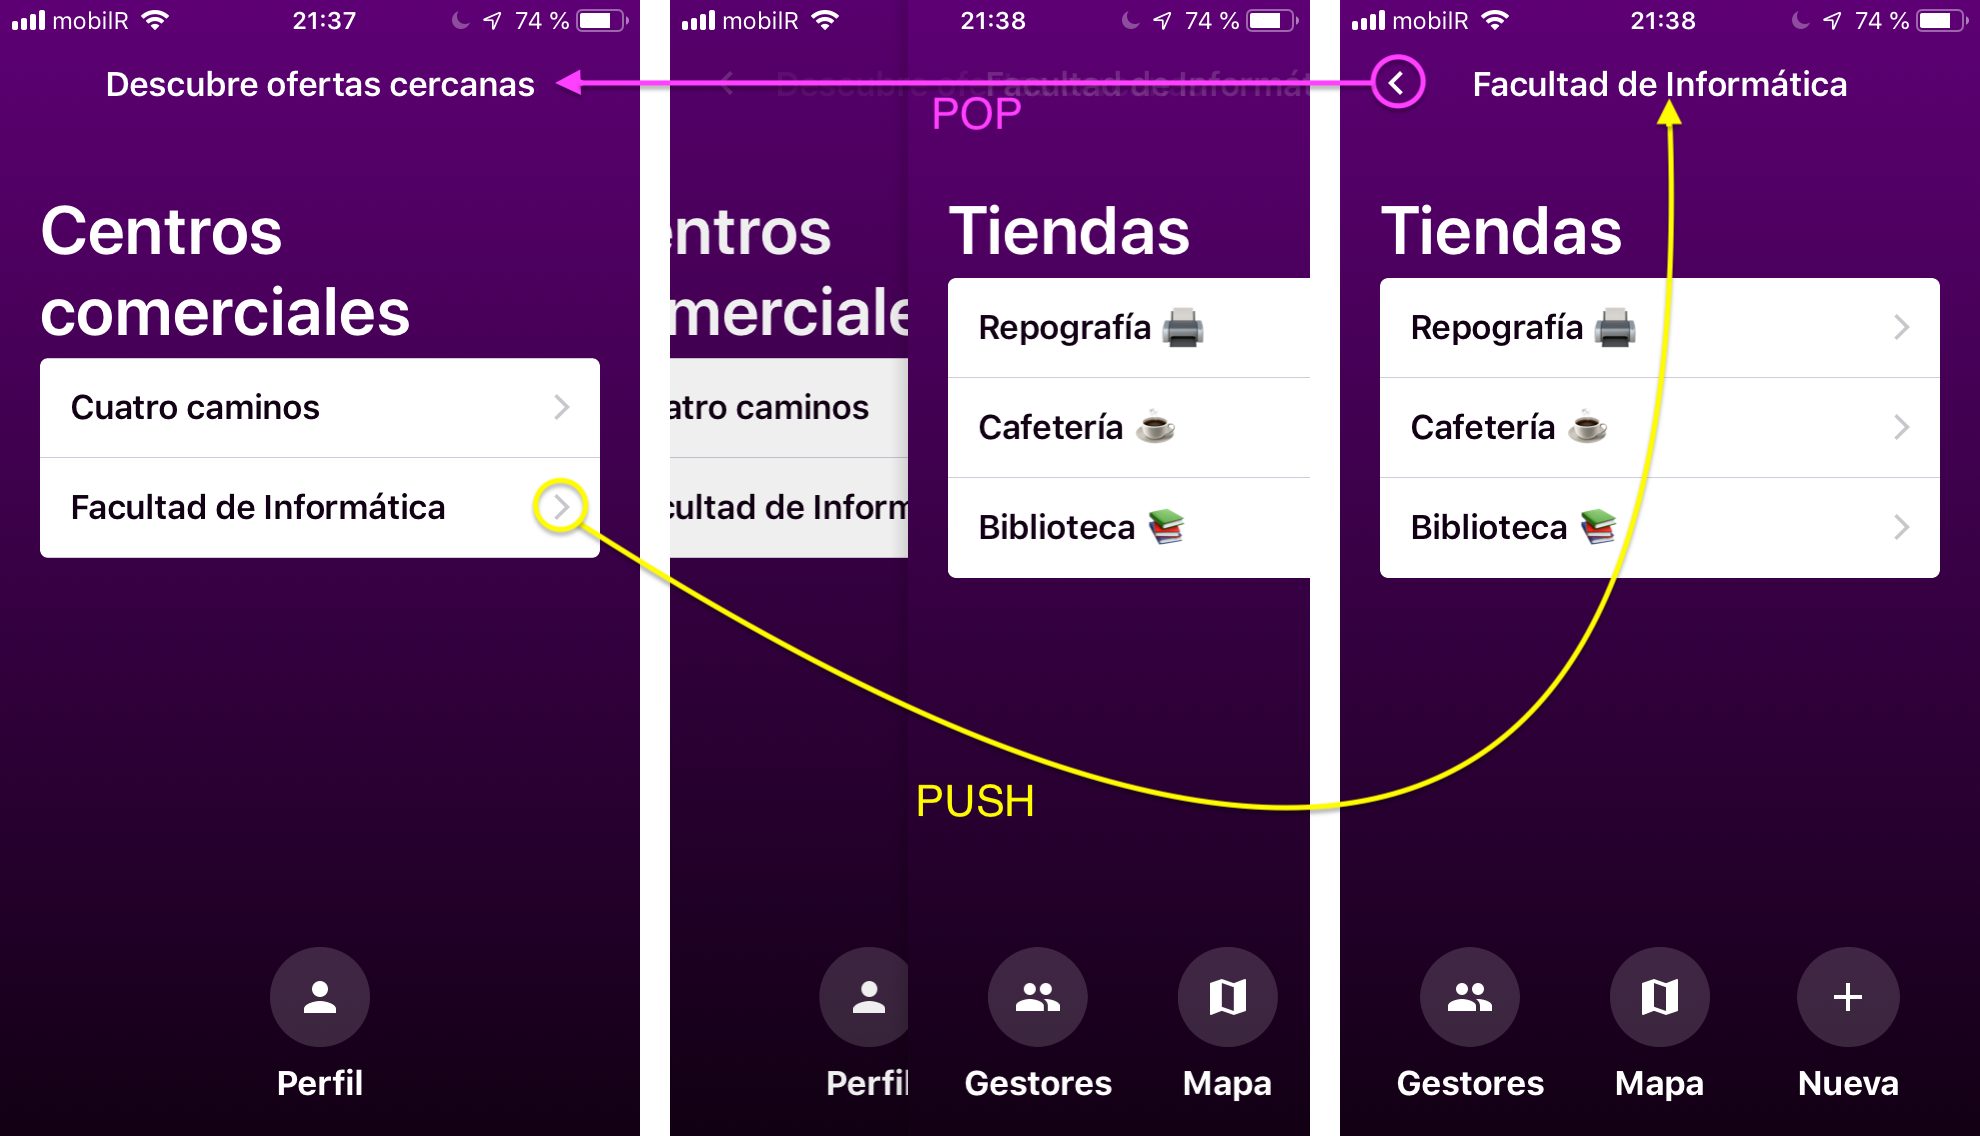
\includegraphics[scale=0.15]{figures/pop-push.png}
\caption{Transiciones entre controladores: \textit{push} y \textit{pop}.\label{ref:pop-push}}
\end{figure}

\subsubsection*{Controladores hijos}\label{contr-hijos}
Serían todos aquellos que no son el \textit{UINavigationController}. Todo controlador tiene asociada una vista, es el controlador quien maneja todas las interactuaciones del usuario con la vista y también es él quien se encarga de mostrarle al usuario a través de la vista todo lo que sea necesario. Una característica que tiene un controlador, es que tiene la capacidad de presentar en pantalla a cualquier otro. Pero a diferencia que con el \textit{UINavigationController}, no va metiendo los nuevos controladores que presenta en una pila, sino que simplemente los muestra y ahí permanecen hasta que se cierran.

Un ejemplo de esto serían las alertas, que también son controladores independientes; presentados por otro controlador que no tiene porque ser un \textit{UINavigationController}, ver figura~\ref{fig:modal}.

\begin{figure}[t]
\centering
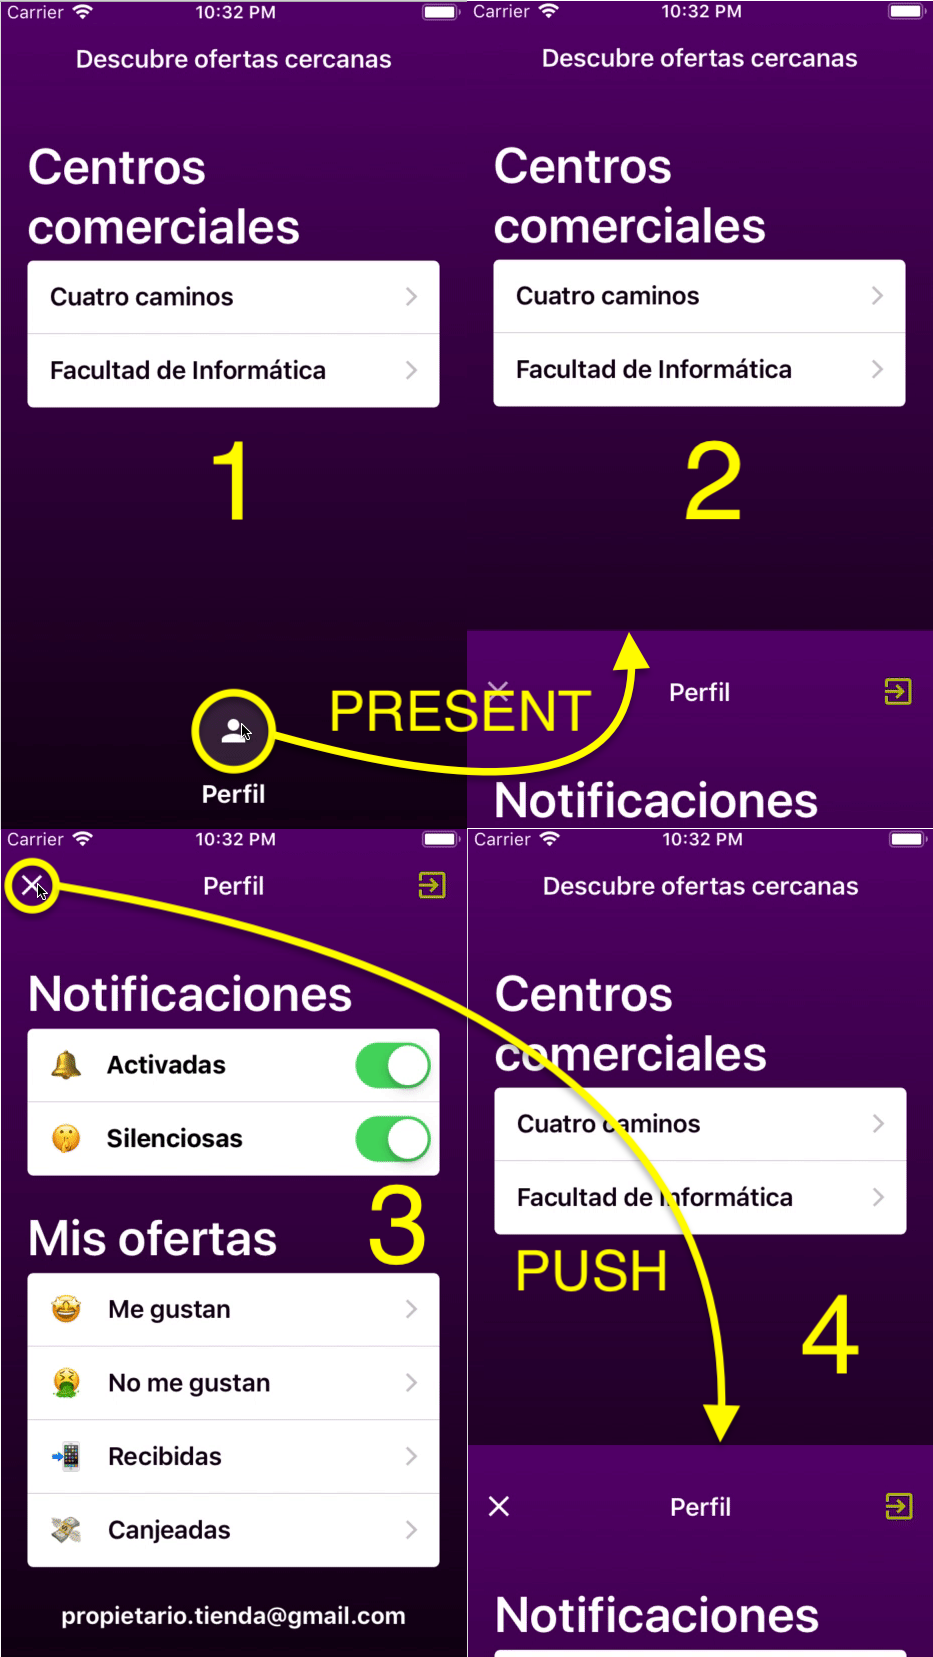
\includegraphics[scale=0.22]{figures/modal.png}
\caption{\textit{Present} para mostrar en pantalla un controlador y \textit{dismiss} para quitarlo.\label{fig:modal}}
\end{figure}

\subsubsection*{Un \textit{UINavigationController} puede ser presentado por otro controlador}
Un controlador normal de los que comentábamos en el apartado \ref{contr-hijos} puede presentar a un controlador padre para que empiece a formar una nueva pila. Puede haber más de un \textit{UINavigationController} y por lo tanto, más de una pila de controladores a la vez, pero sólo uno visible.

